\chapter{System wykrywania kolizji}
\thispagestyle{chapterBeginStyle}
\label{ch:collission_detection}

W tym rodziale opiszę jak działają różne systemy wykrywania kolizji i w jaki sposób niektóre z nich zostały użyte w projekcie.\\

\noindent Są dwa modele wykrywania kolizji:
\begin{itemize}[topsep=0.2em, itemsep=0.5em, partopsep=0em, parsep=0em]
	\item ciągły, w którym ustalamy dokładny moment i miejsce zderzenia
	\item dyskretny, w którym to czy obiekty się zderzyły sprawdzamy co jaki\'s czas
\end{itemize}\bigskip

\noindent{\LARGE Wykrywanie kolizji w modelu ciągłym}

Ten model wykrywania kolizji jest zazwyczaj używany tam, gdzie jest wymagana bardzo duża dokładno\'sć w obliczaniu miejsca i czasu zderzenia. W obliczeniach związanych z tym modelem często używa się interpolacji i metod numerycznych, przez co jest zbyt czasochłonny aby użyć go w progamach działających w czasie rzeczywistym, je\'sli trzeba takie obliczenia wykonać na wielu obiektach. Najczę\'sciej używa się go w symulacjach i modelach fizycznych, a bardzo rzadko w grach. Często model taki musi uwzględniać informacje o parametrach fizycznych obiektów takich jak ich elastyczno\'sć, oraz to jak obiekt będzie się poruszał według zasad fizyki.\\

\begin{figure}[h]
	\centering
	\noindent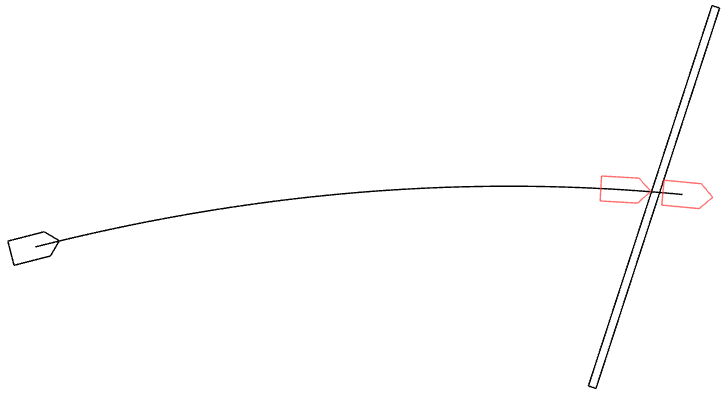
\includegraphics[width=0.8\textwidth]{collission_detection_continuous}
	\caption{Wykrywanie kolizji w modelu ciągłym, punkt wej\'scia dla t=60.947, punkt wyj\'scia dla t=66.563}
\end{figure}
\newpage
\noindent{\LARGE Wykrywanie kolizji w modelu dyskretnym}

Ten model wykrywania kolizji jest używany wszędzie, gdzie nie jest wymagana taka dokładno\'sć jak przy trybie ciągłym. Polega on na sprawdzaniu czy obiekty kolidują co jaki\'s okres czasu, zazwyczaj co cykl obliczeń zmieniających położenie obiektów. Jest dużo prostszy i wymaga dużo mniej obliczeń, dlatego mozna go używać w czasie rzeczywistym na wielu obiektach naraz. Najczę\'sciej jest on używany w grach albo prostych symulacjach, niewymagających dużej dokładno\'sci. Do algorytmów używających tego modelu nie trzeba też wysyłać tylu informacji, wystarczy podać mu listę modeli, na których chcemy sprawdzić, czy zaszły zderzenia.\\

\begin{figure}[h]
	\centering
	\noindent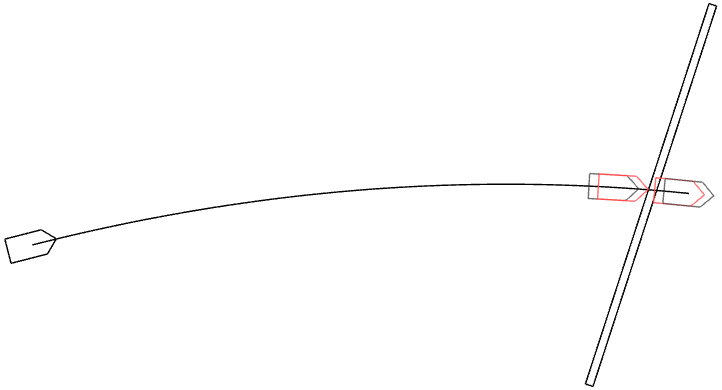
\includegraphics[width=0.8\textwidth]{collission_detection_discrete}
	\caption{Wykrywanie kolizji w trybie dyskretnym, zderzenie następuje między klatkami 61 i 66}
\end{figure}

Jego minusem jest jednak to że prędko\'sci obiektów muszą być dopasowane do ich wielko\'sci, je\'sli mały obiekt porusza się bardzo szybko to zderzenie może nie zaj\'sć, ponieważ w jednym cyklu obliczeń obiekt będzie całkowicie przed, a w drugim całkowicie za przeszkodą.\\

\begin{figure}[h]
	\centering
	\noindent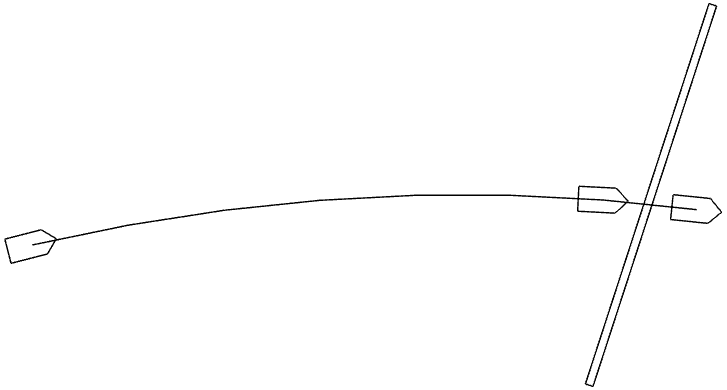
\includegraphics[width=0.8\textwidth]{collission_detection_discrete_problem}
	\caption{Problem z wykrywaniem kolizji w trybie dyskretnym przy zbyt duzym odstępie między obliczeniami, w takim przypadku zderzenie między obiektami nie zostaje zarejestrowane}
\end{figure}
\newpage

\noindent W moim projekcie zastosowałem model dyskretny, ponieważ nie jest tu wymagana taka duża dokładno\'sć i pasuje on do sposobu w jaki działa silnik gry (wykonywanie aktualizacji co pewien okres).\\

\noindent Wykrywanie kolizji dzieli się na dwie fazy:\begin{itemize}[topsep=0.2em, itemsep=0.5em, partopsep=0em, parsep=0em]
	\item Broad phase
	\item Narrow phase
\end{itemize}\bigskip

\noindent{\Huge Broad Phase}

W tej fazie wykrywa się jak najwięcej par obiektów, które na pewno się ze sobą nie zderzą, ponieważ np. są daleko od siebie. Obliczenia w tej fazie powinny być jak najprostsze, aby szybko i skutecznie odrzucić dużo par obiektów.

Algorytmy najczę\'sciej używane podczas Broad phase dzielą się na te, które dzielą lub układają przestrzeń i te, które po prostu porównują każdy obiekt z każdym poprzez otoczenie go jakim\'s kształtem.\\
Algorytmy, które opiszę, to:\begin{itemize}[topsep=0.2em, itemsep=0.5em, partopsep=0em, parsep=0em]
	\item AABB (Axis-Aligned Bounding Boxes)
	\item Bounding Boxes
	\item Bounding Circles
	\item Sweep and Prune
	\item Quadtree
	\item Octree
	\item Bounding Volume Hierarchy
	\item Bins
\end{itemize}
\bigskip
\noindent Czasami można w tej fazie użyć tymczasowej koherencji, czyli skorzystać z faktu, iż niektóre obiekty nie przesunęły się względem siebie od czasu ostatniego wykrywania kolizji, lub przesunęły się o względnie małą odległo\'sć, dzięki czemu od razu można je wykluczyć.\\

\noindent{\LARGE Bounding Volumes}\smallskip

Metody z grupy Bounding Volumes polegają na otoczeniu modelu jakim\'s prostym kształtem, i sprawdzaniu zderzeń tylko na tych kształtach. Są zazwyczej do\'sć proste do zaimplementowania i bardzo dobre je\'sli obiektów jest mało.\\

\noindent{\LARGE Space Partitioning}\smallskip

Druga grupa metod, wykorzystują one podział pola gry na obszary, zazwyczaj ułożone w strukturę drzewa. W każdym z pól każda para obiektów dla danego pola zostaje przetestowana czy została zderzona. Podział na obszary można zaimplementować na wiele sposobów.

\newpage
\noindent{\Large AABB (Axis-Aligned Bounding Boxes)}\smallskip

Metoda AABB polega na otoczeniu każdego obiektu prostokątem i sprawdzeniu które prostokąty się pokrywają.

Zaletami tej metody są łatwo\'sć implementacji, a także dokładno\'sć dla obiektów przypominających kształtem prostokąty wyrównane do osi.

Wadami tej metody są czas działania, czyli $O(n^{2})$ dla $n$ elementów, oraz fakt że dla pewnych obiektów jest ona bardzo niedokładna. Dla obracających lub zmieniających rozmiar obiektów trzeba też zmienić rozmiar prostokąta, co czasami może wymagać dużej ilo\'sci obliczeń, je\'sli model ma wiele wierzchołków.\\
Metody tej najlepiej używać, gdy obiektów jest niewiele i są one prostokątne (na przykład w platformówkach).
\begin{figure}[h]
	\centering
	\noindent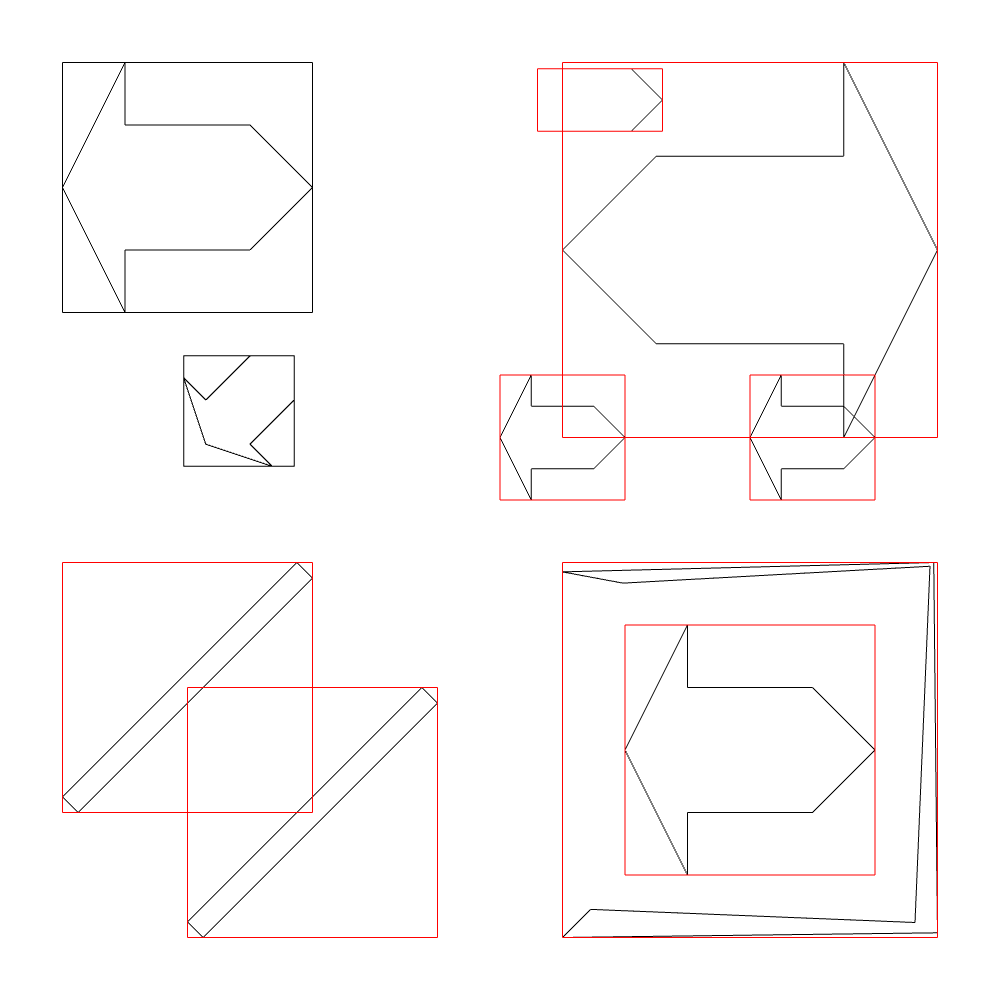
\includegraphics[width=0.84\textwidth]{collissionAABB}
	\caption{Przykład wykrywania kolizji metodą AABB, kolidujące obiekty są oznaczone na czerwono}
\end{figure}\\
Jak widać na obrazku, większo\'sć obiektów z czym\'s koliduje, ale pary obiektów będących daleko od siebie są odrzucone, co zdecydowanie zmniejsza liczbę obliczeń.
\newpage

\noindent{\Large Bounding Boxes}\smallskip

Ta metoda polega na otoczeniu każdego obiektu prostokątem, który nie musi być wyrównany do osi, w innych aspektach jest podobna do poprzedniej. Jest ona odrobinę trudniejsza do zaimplementowania, ale dzięki możliw\'soci obracania może być także dokładniejsza w niektórych przypadkach, a przy obrocie obiektu wystarczy obrócić odpowiadający mu prostokąt.

Wady tej metody to nieco większa złożono\'sć obliczeń, ciągle przy $O(n^{2})$ porównań.
\begin{figure}[h]
	\centering
	\noindent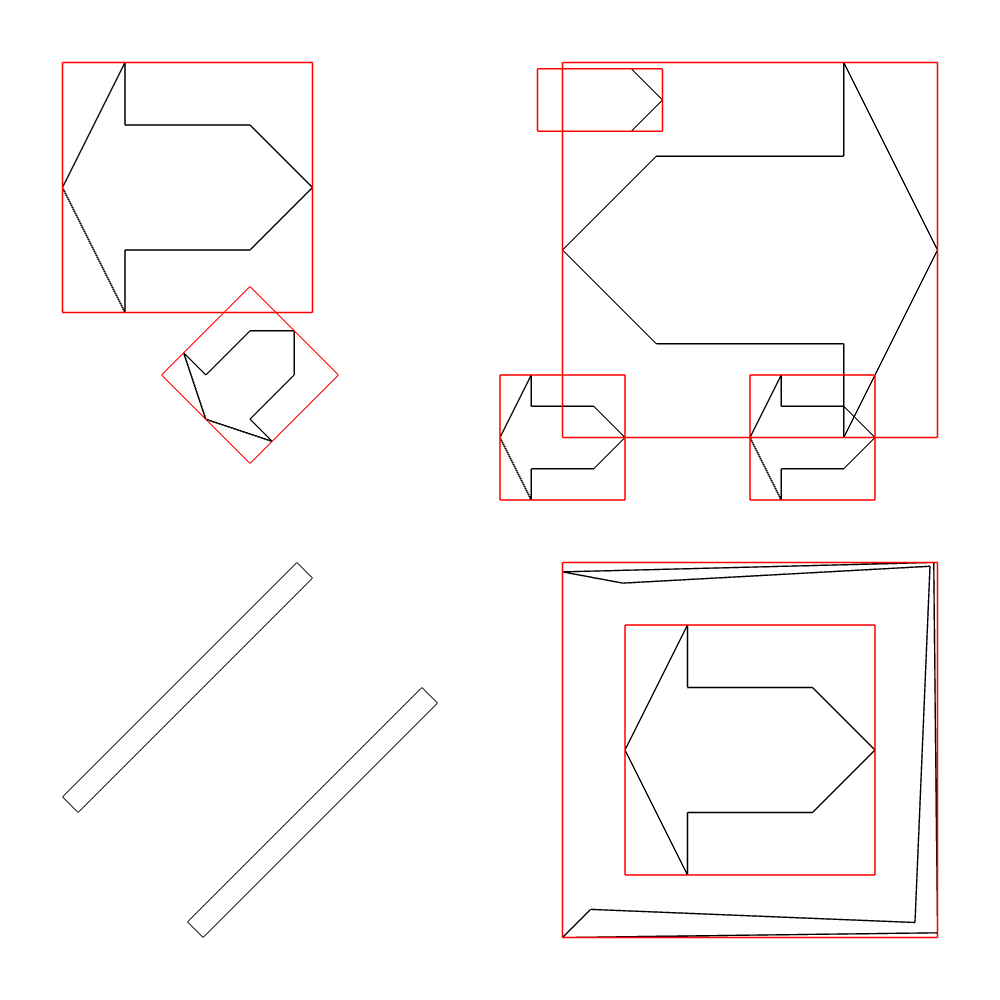
\includegraphics[width=\textwidth]{collission_rotated_boxes}
	\caption{Przykład wykrywania kolizji metodą Bounding Boxes}
\end{figure}\\
Patrząc na obrazek, w lewym dolnym rogu prostokąty odpowiadają teraz modelowi obiektu, ale za to w lewym górnym rogu widać, że tym razem program wykrył kolizję, której nie było w poprzednim przykładzie.
\newpage

\noindent{\Large Bounding Circles}\smallskip

Ta metoda jest podobna do dwóch poprzednich, ale tym razem używamy koła do sprawdzania możliwych zderzeń.

Plusami tej metody są łatwo\'sć jej zaimplementowania i bardzo mała ilo\'sć wymaganych danych oraz obliczeń: wystarczy tylko obliczyć odległo\'sc między dwoma obiektami i porównać z sumą ich promieni. Dodatkowo obrót obiektów i ich skalowanie nie wymusza obliczania danych na nowo, jesli używamy tej metody.

Wady tej metody to kiepska wydajno\'sć dla obiektów które są podłużne.
\begin{figure}[h]
	\centering
	\noindent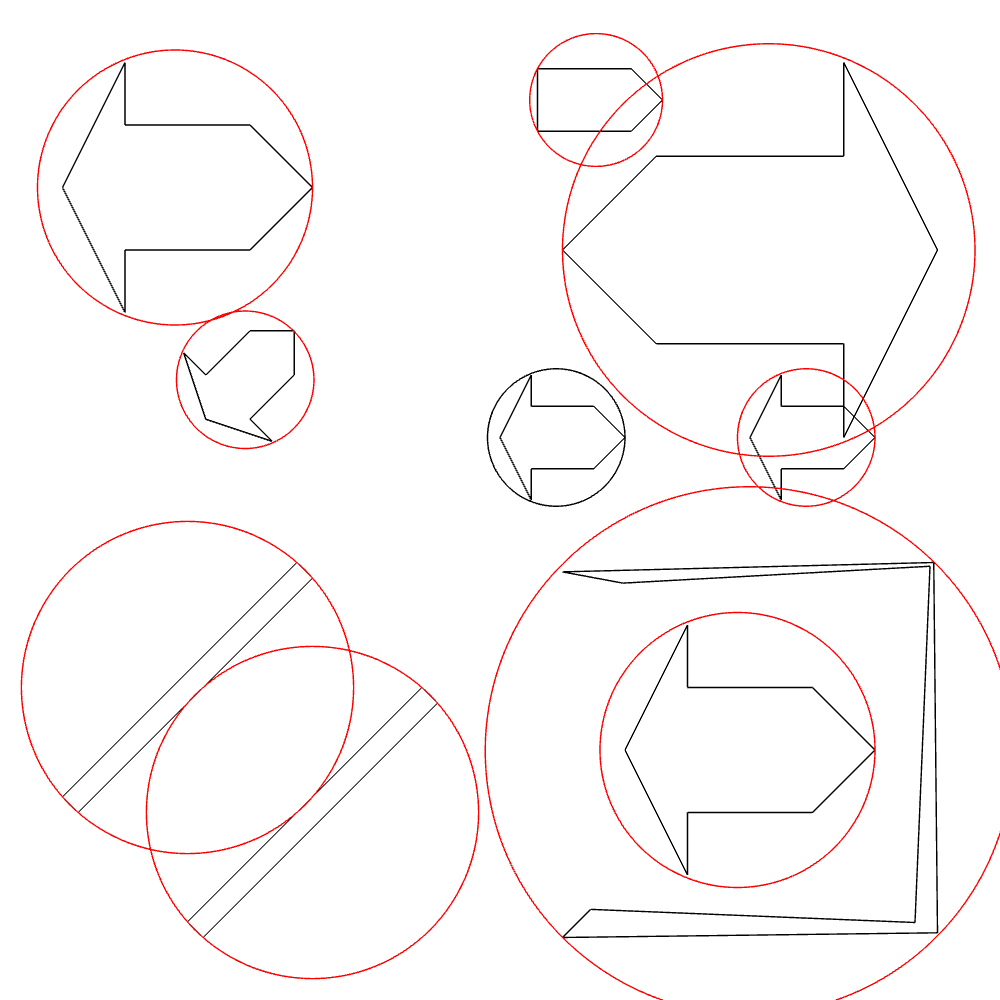
\includegraphics[width=\textwidth]{collission_circles}
	\caption{Przykład wykrywania kolizji metodą Bounding Circles}
\end{figure}\\
\newpage

\noindent{\Large Sweep and Prune}\smallskip

Metoda polegająca na posortowaniu obiektów względem położenia na osiach tych ich punktów, które są najbliżej i najdalej początku osi. Potem je\'sli początki i końce danej pary nakładają się na wszystkich osiach, to ta para przechodzi dany etap.

Zalety tej metody to szybszy czas działania, $O(nlogn)$ w porównianiu do $O(n^{2})$ poprzedniej metody.
\begin{figure}[h]
	\centering
	\noindent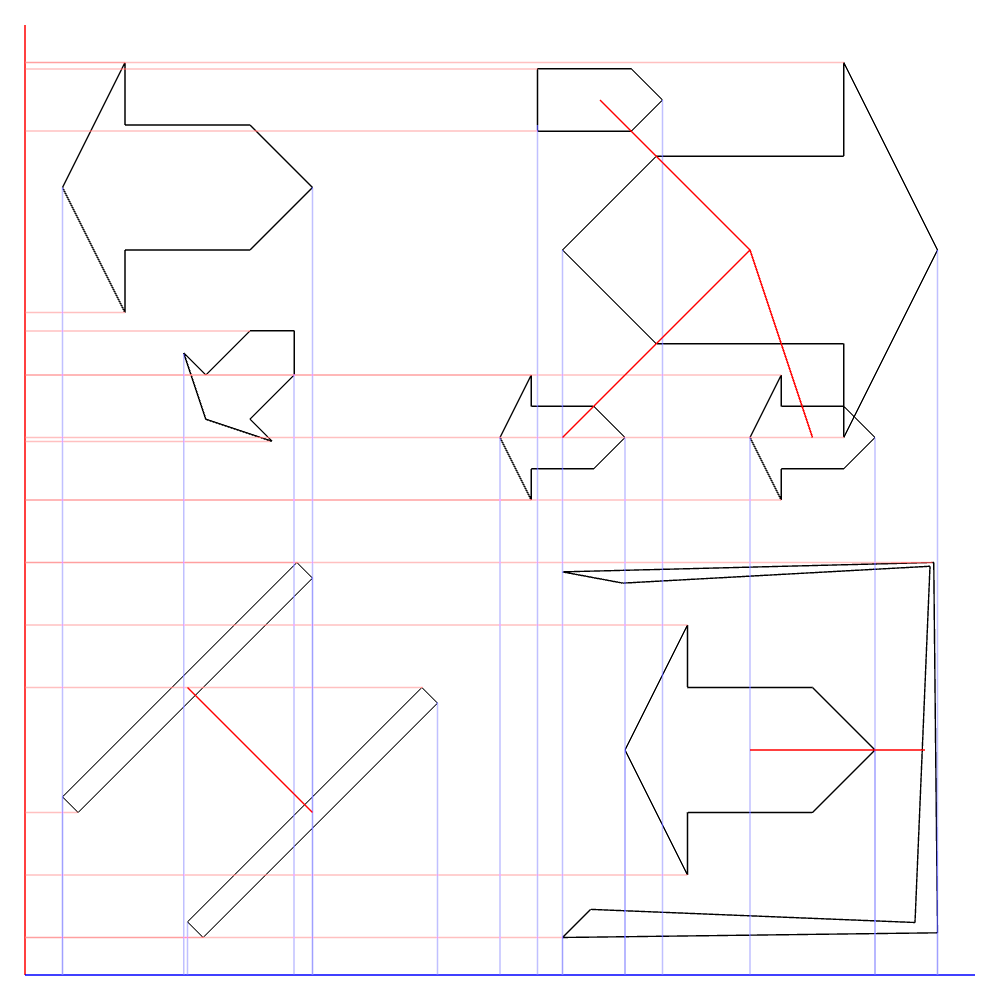
\includegraphics[width=\textwidth]{collission_sweep_and_prune}
	\caption{Przykład wykrywania kolizji metodą Sweep and Prune, kolizje są oznaczone czerwoną linią}
\end{figure}\\
Jak widać na obrazku, Wyniki są dokładnie takie same jak dla metody AABB, jednak czas działania tej metody jest dużo krótszy je\'sli niewiele elementów ze sobą koliduje.
\newpage

\noindent{\Large Quadtree}\smallskip

Każdy obszar jest kwadratem i może być podzielony na 4 podobszary, je\'sli zawiera odpowiednio małe elementy. Wykrywanie kolizji zachodzi gdy w jednym obszarze znajduje się więcej niż jeden obiekt.\\
\begin{figure}[h]
	\centering
	\noindent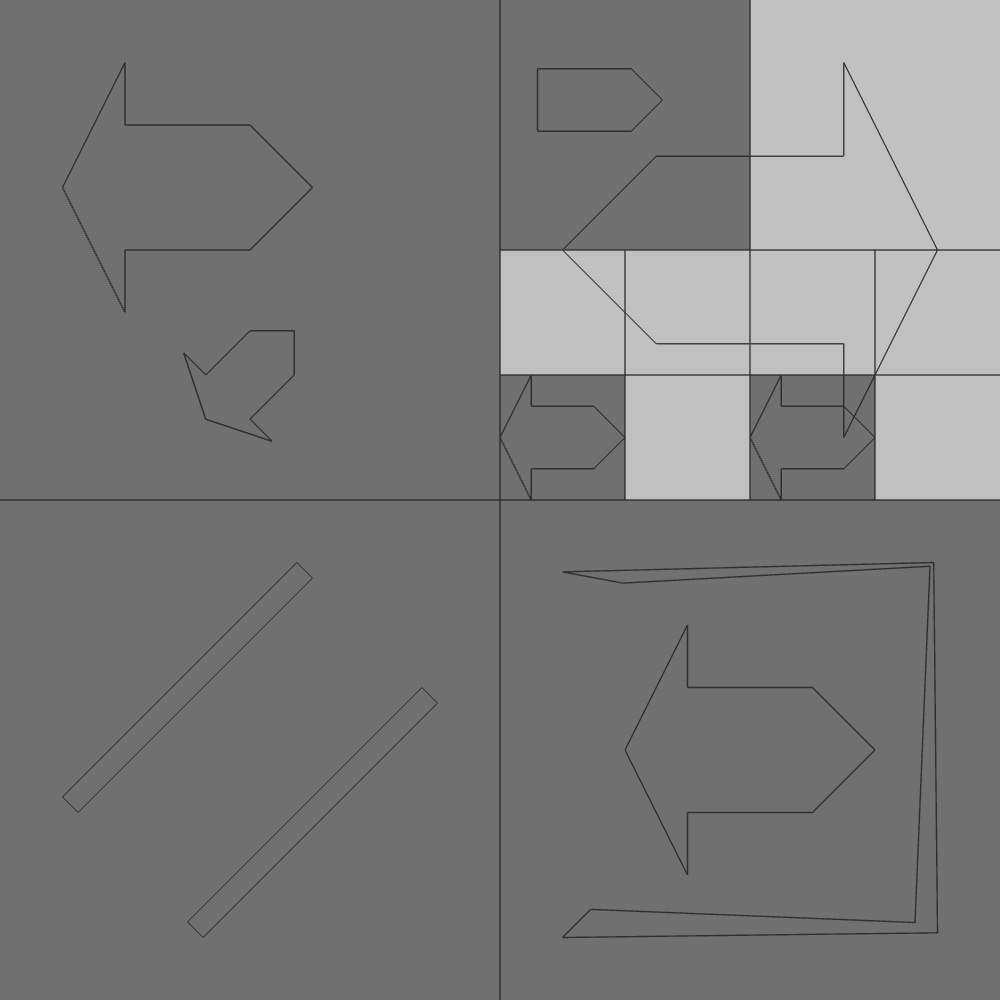
\includegraphics[width=\textwidth]{collission_quadtree}
	\caption{Przykład użycia metody Quadtree}
\end{figure}\\

\noindent{\Large Octree}\smallskip

Podobnie jak w Quadtree, Octree dzieli obszar na równej wielko\'sci podobszary, z tym że tutaj podział następuje w przestrzeni trójwymiarowej, sze\'scian dzieli się na 8 mniejszych sze\'scianów.\\
\newpage
 
\noindent{\Large Bounding Volume Hierarchy}\smallskip

Ta metoda tworzy drzewo przez połączenie dwóch drzew będących blisko siebie w jedno większe drzewo, którego będą poddrzewami. Obydwa poddrzewaw cało\'sci mieszzcą się w obszarze będącym korzeniem drzewa. Tutaj kolizje zachodzą, je\'sli dwa poddrzewa się na siebie nakładają.\\
\begin{figure}[h]
	\centering
	\noindent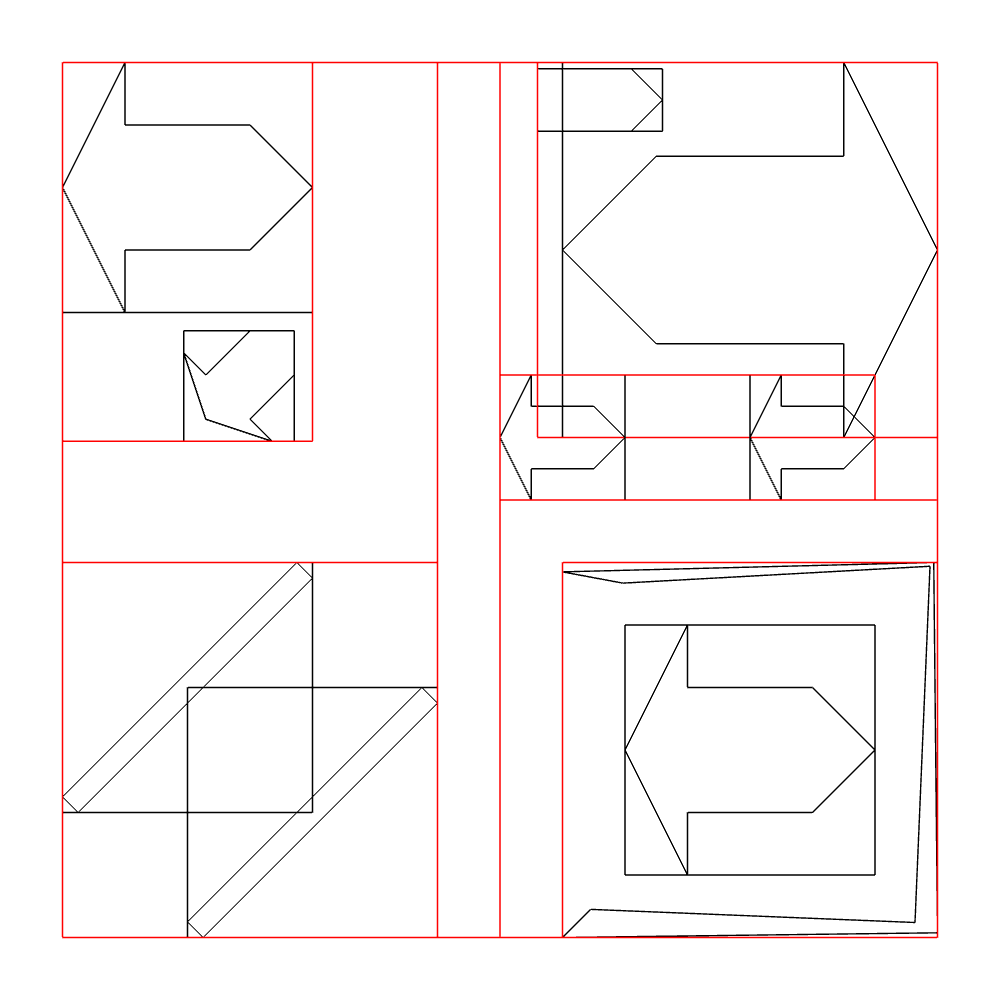
\includegraphics[width=\textwidth]{collission_bounding_volumes_hierarchy}
	\caption{Przykład użycia metody Bounding Volume Hierarchy}
\end{figure}\\
\newpage

\noindent{\Large Bins}\smallskip

Najprostsza z metod opartych na dzieleniu obszaru. Metoda ta dzieli obszar na wiele równych czę\'sci i do każdej z nich dodaje wszystkie obiekty które się z nią chociaż czę\'sciowo pokrywają. W danym obszarze kolizje liczone są w parach obiektów każdy z każdym.\\
\begin{figure}[h]
	\centering
	\noindent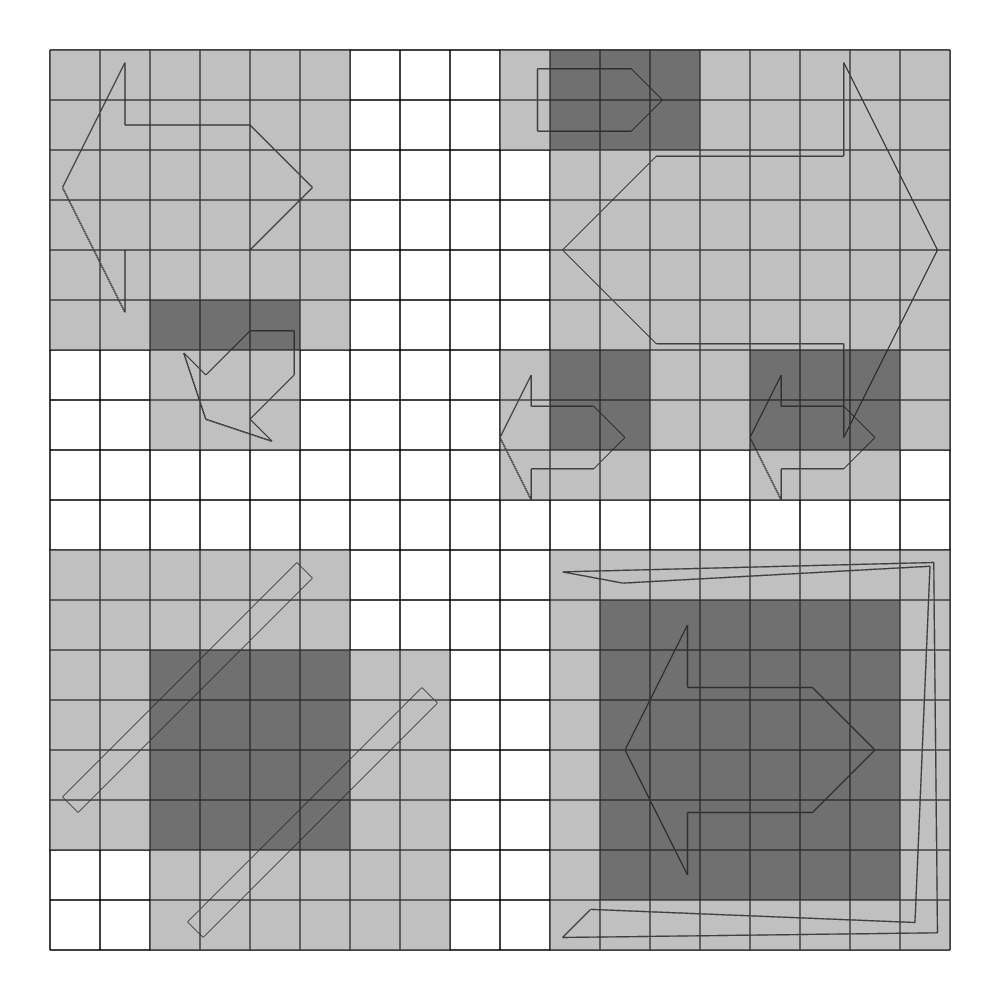
\includegraphics[width=\textwidth]{collission_bins}
	\caption{Przykład użycia metody , im pole ciemniejsze, tym więcej obiektów je pokrywa}
\end{figure}\\
\newpage

W projekcie została użyta metoda Bounding Circles, ze względu na to, że obiekty w grze często się obracają i mają w wielu przypadkach kształt zbliżony do koła. Aby zmniejszyć liczbę obliczeń, obiekty zostały podzielone na kategorie.\\

\noindent Obiekty podzielone są na następujące kategorie:\begin{itemize}[topsep=0.2em, itemsep=0.5em, partopsep=0em, parsep=0em]
	\item przeciwnicy
	\item pociski przeciwników
	\item gracz
	\item pociski gracza
	\item teren i tło
	\item inne
\end{itemize}

\noindent Dzięki takiemu podziałowi można uniknąć obliczeń między obiektami które nie mają się ze sobą zderzać ani wchodzić w interakcję, a także wybierać z obiektami jakich kategorii dany obiekt może wchodzić w interakcje.\\
Po przej\'sciu przez etap Broad Phase, pozostałe pary obiektów zostają następnie przeniesione do drugiego etapu, którym jest Narrow Phase.\\

\noindent{\Huge Narrow Phase}

Ta faza polega na dokładnym wykryciu kolizji pomiędzy obiektami i pewną odpowiedzią czy obiekty kolidują czy też nie. Obliczenia w tej fazie powinny być tak dokładne jak to możliwe.\\

\noindent{\Large Wykrywanie kolizji metodą Pixel Perfect Collission Detection}\smallskip

Ta metoda jest używana zazwyczaj w grach dwuwymiarowych, gdzie model można przedstawić w postaci siatki pikseli, na której każdy piksel ma dwa kolory, jeden przedstawiający zawieranie się danego piksela w modelu obiektu i drugi w przeciwnym przypadku, zazwyczaj czarny.

Testowanie kolizji dwóch obiektów polega na nałożeniu odpowiednio przesuniętych siatek obu obiektów na siebie i sprawdzeniu, czy istnieją piksele w których kolor obu modeli się pokrywa.

Obliczenia te można do\'sć łatwo wykonać na wielu wątkach jednocze\'snie, czasami były one też wspomagane sprzętowo. W dzisiejszych czasach to rozwiązanie jest jednak do\'sć rzadko spotykane.

Można zasymulować tą metodę przy pomocy odpowiednio napisanej funkcji rysującej modele na buforze, a następnie sprawdzeniu czy bufor zawiera piksel w danym kolorze. Możliwe jest wtedy użycie do rysowania np. karty graficznej, co znacznie przyspieszyłoby obliczenia.\bigskip

Poniżej jest napisany w pseudokodzie przykładowy algorytm sprawdzania zderzenia między dwoma obiektami.\\
Siatki składają się z pikseli, zawierających swoje położenie oraz warto\'sć, 1 je\'sli piksel należy, a 0 je\'sli nie należy do modelu.\\
Na początku algorytmu tworzony jest odpowiednio duży bufor wypełniony zerami.\\
Następnie bufor jest wypełniany jedynkami tam, gdzie pierwsza siatka ma wypełnione piksele.\\
To samo zostaje powtórzone dla drugiej siatki, z tym, że teraz zamiast ustawiać warto\'sć na 1, wykonujemy operację AND, dzięki czemu piksele będą miały warto\'sć 1 tylko tam, gdzie modele się zderzają, piksele drugiej siatki są też przesunięte.\\
Na koniec zostaje sprawdzone, czy którykolwiek z pikseli bufora ma warto\'sć 1, je\'sli tak, to zostaje zwrócona warto\'sć true, w przeciwnym wypadku zostaje zwrócona warto\'sć false.\bigskip

\noindent Obrazek \ref{pixel_perfect} ilustruje przykład użycia tej metody, pierwszy obiekt jest narysowany na czerwono, a drugi na niebiesko, miejsce zderzenia jest oznaczone przez fioletowe pola. W przypadku, gdyby nie było takich pól, oznaczałoby to, że kolizja nie zaszła.
\newpage
\begin{algorithm}[H]
	\KwIn{$m_1$ - siatka pierwszego obiektu\\ $m_2$ - siatka drugiego obiektu\\ $x, y$ - przesunięcie drugiego obiektu względem pierwszego}
	\KwOut{warto\'sć typu boolean, mówiąca czy obiekty się zderzyły czy też nie}
	\Begin{
		xMin $\leftarrow$ min(0, x);\\
		xMax $\leftarrow$ max($m_1$.width-1, $m_2$.width+x-1);\\
		yMin $\leftarrow$ min(0, y);\\
		xMax $\leftarrow$ max($m_1$.height-1, $m_2$.height+y-1);\\
		test $\leftarrow$ new ArrayOfZeroes[xMin..xMax][[yMin..yMax];\\
		\ForEach{pixel in $m_1$}{
			\If{pixel.val == 1 }{
				test[pixel.x][pixel.y] $\leftarrow$ 1;
			}			
		}
		\ForEach{pixel in $m_2$}{
			test[pixel.x][pixel.y] $\leftarrow$ test[x+pixel.x][y+pixel.y] AND pixel.val;
		}
		\ForEach{pixel in test}{
			\If{pixel == 1 }{
				return true;
			}
		}
		return false;
	}
	\caption{Algorytm wykrywający kolizję dwóch modeli metodą Pixel Perfect Collission Detection}
\end{algorithm}\bigskip
\begin{figure}[h]
	\centering
	\noindent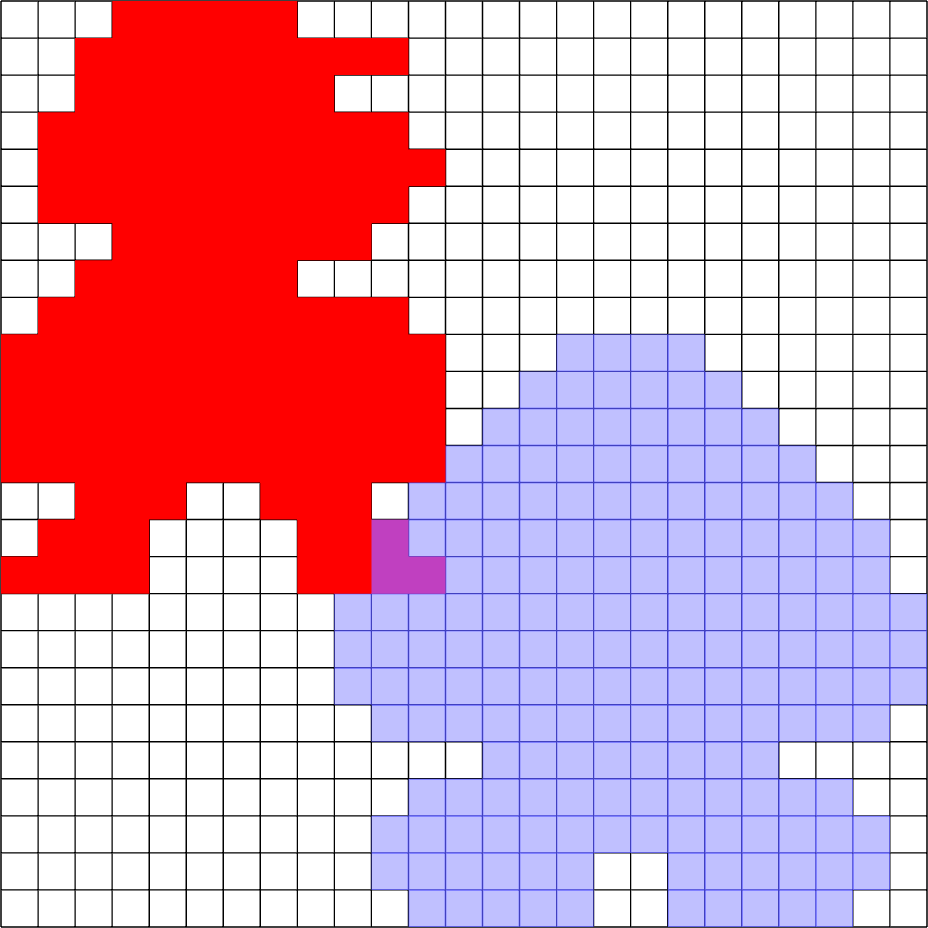
\includegraphics[width=0.65\textwidth]{collission_pixel_perfect}
	\caption{Przykład Pixel Perfect Collission Detection}
	\label{pixel_perfect}
\end{figure}
\newpage

\noindent{\Large Wykrywanie kolizji metodą Separating Planes}\smallskip

Metoda Płaszczyzn Oddzielających polega na znalezieniu płaszczyzny, która oddziela od siebie dwa obiekty.
Płaszczyzna taka istnieje je\'sli są spełnione następujące warunki:
\begin{itemize}[topsep=0.2em, itemsep=0.5em, partopsep=0em, parsep=0em]
	\item Zbiory punktów należących do obydwu obiektów są zbiorami wypukłymi
	\item Obiekty się nie pokrywają
\end{itemize}\bigskip

\noindent Zbiór wypukły to taki zbiór, w którym odcinek łączący dowolne dwa punkty ze zbioru, także znajduje się w cało\'sci w tym zbiorze.\\
Otoczka wypukła to najmniejszy zbiór wypukły, który zawiera cały dany zbiór, może być równa temu zbiorowi.\\
Aby zbiór utworzony z powierzchni danego modelu mógł być zbiorem wypukłym (czyli aby model był równy swojej otoczce wypukłej), model taki musi być wielokątem wypukłym, czyli kąt wewnętrzny między dowolnymi dwiema sąsiadującymi krawędziami musi być mniejszy lub równy $\Pi$ radianów.\\
Je\'sli modele obu zderzanych obiektów są otoczkami wypukłymi, to obiekty nie zderzają się ze sobą wtedy i tylko wtedy, gdy istnieje płaszczyzna oddzielająca te dwa modele.\\
Jednak co zrobić, gdy model nie jest równy swojej otoczce wypukłej?\\
Są na to dwa rozwiązania:
\begin{itemize}
	\item stworzyć dla modelu jego otoczkę wypukłą i uzywać jej do obliczeń
	\item podzielić model tak, aby każda jego czę\'sć była otoczką wypukłą
\end{itemize}

Minusem pierwszego rozwiązania jest niedokładno\'sć, wynikająca z dodania do pola modelu dodatkowej przestrzeni aby zrobić z niego zbiór wypukły. Plusem jest to, że liczba wierzchołków do przetworzenia się zmniejsza, ponieważ trzeba tylko pousuwać te wierzchołki, w których kąt wewnętrzny jest większy niż $2\Pi$ radianów.

Minusem drugiego rozwiązania jest zwiększenie mocy obliczeniowej potrzebnej do policzenia nowego modelu oraz wykrycie zderzenia na większej ilo\'sci wierzchołków. Plusem jest dokładno\'sć, ta metoda jest tak dokładna jak oryginalny model.\\

Jest wiele algorytmów tworzących z modelu jego otoczkę wypukłą. W projekcie został zaimplementowany algorytm skanu Grahama, przedstawiony poniżej.\\

\begin{algorithm}[H]
	\KwIn{m - lista punktów należących do modelu}
	\KwOut{lista punktów tworzących otoczkę wypukłą danego modelu}
	\Begin{
		p $\leftarrow$ m[0];\\
		\ForEach{point in m}{
			\If{point.y\textless p.y OR (point.y == p.y AND point.x\textless p.x) }{
				p $\leftarrow$ point;
			}
		}
		pointList $\leftarrow$ sortByPolarAngle(m, p);\\
		insertInFront(pointList, p);\\
		i $\leftarrow$ 0;\\
		\While{i \textless  pointList.size}{
			p1 $\leftarrow$ pointList[i];\\
			p2 $\leftarrow$ pointList[mod(i+1, pointList.size)];\\
			p3 $\leftarrow$ pointList[mod(i+2, pointList.size)];\\
			\eIf{polarAngle(p1, p2)\textless polarAngle(p2, p3)}{
				i++;
			}{
				deleteElementFromList(pointList, mod(i+1, pointList.size));
			}	
		}
		return pointList;
	}
	\caption{Algorytm tworzący otoczkę wypukłą z danych punktów}
\end{algorithm}\bigskip

\noindent Powyższy algorytm przyjmuje na wej\'sciu listę punktów tworzących model.

Pierwszy etap algorytmu to znalezienie punktu położonego najniżej na osi Y, a je\'sli jest takich kilka to także przesuniętego najbardziej w lewo na osi X. Punkt ten będzie pierwszym punktem należącym do otoczki, nazwijmy go p.

Następnie algorytm sortuje wszystkie inne punkty według ich kąta polarnego względem punktu p. Po posortowaniu punkt p jest dodawany na początek listy.

Ostatnim etapem algorytmu jest usunięcie punktów, które nie tworzą otoczki. Punkty takie można rozpoznać po tym, że je\'sli przechodzimy listę, to idąc po krawędzi łączącej dany punkt z poprzednim musimy skręcić zgodnie z ruchem wskazówek zegara, aby przej\'sć na krawędź łączącą dany punkt z następnym. Wszystkie takie punkty usuwamy z listy, pozostałe dla których skręcamy przeciwnie do ruchu wskazówek zegara, zostawiamy na li\'scie.

Wynikiem jest lista punktów tworzących otoczkę wypukłą danego modelu.

Złożono\'sć algorytmu dla n punktów to O(n) dla pierwszego etapu (wybierania początkowego punktu), O(nlogn) dla sortowania oraz O(n) dla przej\'scia po li\'scie i usunięcia niepotrzebnych wierzchołków. Algorytm jest więc ograniczony przez czas sortowania, O(nlogn). Złożono\'sć pamięciowa algorytmu to O(n).

Istnieją algorytmy rozwiązujące ten problem w czasie O(nlogh), gdzie h to ilo\'sć punktów w wyj\'sciowym modelu, są to więc algorytmy, których czas działania jest zależny od wielko\'sci wyj\'scia.\bigskip

Użycie drugiego rozwiązania sprowadza się zazwyczaj do problemu triangulacji wielokąta, z czasem O(nlogn) dla najlepszych algorytmów. W projekcie zostało jednak użyte pierwsze rozwiązanie dla skomplikowanych modeli, a dla mniejszych modeli dane są tworzone ręcznie przy tworzeniu modelu.\bigskip

\noindent{\Large Testowanie kolizji}\smallskip

\noindent Gdy obiekty są już w postaci otoczek wypukłych, można przej\'sć do sprawdzenia czy zaszło zderzenie.\\
Algorytm wyrażony w pseudokodzie wygląda następująco:\begin{enumerate}
	\item dla każdego punktu z pierwszego obiektu:\begin{enumerate}
		\item wyznacz wektor $v$ od danego punktu do następnego punktu w modelu
		\item weź dowolną prostą $p$, która nie jest równoległa do wektora $v$
		\item wykonaj rzut równoległy do wektora $v$ obu obiektów na prostą $p$, otrzymując dwa odcinki na tej prostej, $m_1$ i $m_2$
		\item je\'sli $m_1$ i $m_2$ się nie pokrywają, została znaleziona prosta oddzielająca oba obiekty (równoległa do $v$), następuje koniec algorytmu
	\end{enumerate}
	\item powtórz obliczenia zamieniając obiekty ze sobą
	\item je\'sli nie została znaleziona płaszczyzna oddzielająca, obiekty się pokrywają, koniec algorytmu
\end{enumerate}\bigskip

\noindent Wynikiem tego algorytmu jest pewna odpowiedź czy obiekty kolidują, czy też nie.\\
Złożono\'sć algorytmu, dla wielko\'sci modeli wynoszących $n_1$ i $n_2$, wynosi O($(n_1+n_2)^2$).\newpage

\begin{figure}[h]
	\centering
	\noindent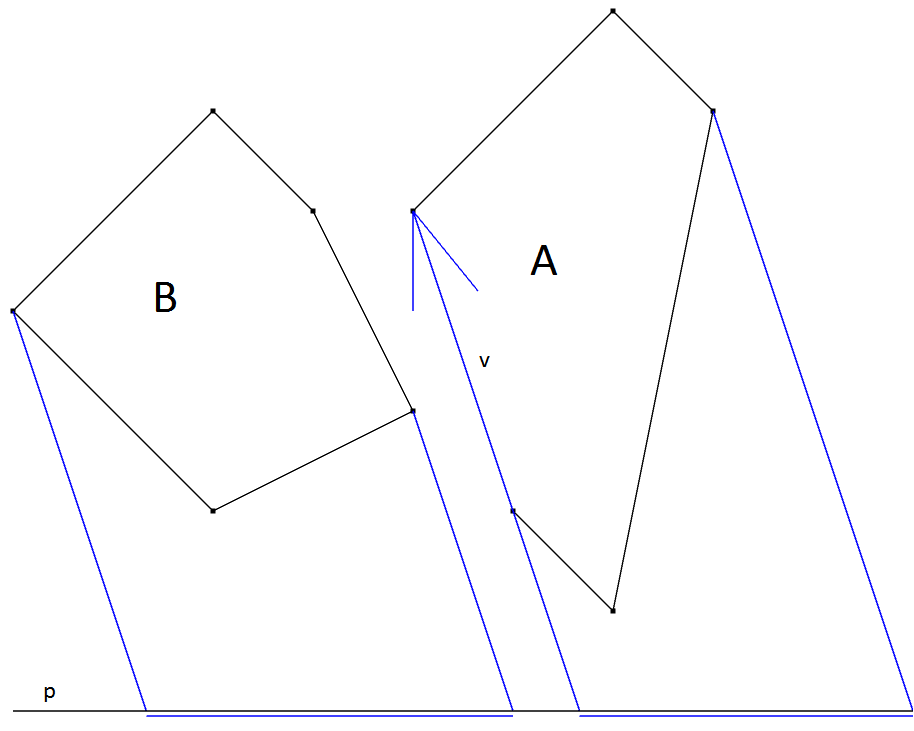
\includegraphics[width=\textwidth]{collission_separating_planes}
	\caption{Przykład wykrywania kolizji metodą płaszczyzn oddzielających, }
	\label{separating_planes}
\end{figure}

Jak widać na obrazku \ref{separating_planes}, obiekty A i B mają płaszczyznę oddzielającą równoległą do $v$, ponieważ ich rzuty na prostą $p$ nie pokrywają się. Dla A i C żadna płaszczyzna równoległa do $v$ nie oddziela tych obiektów, w kolejnym cyklu pętli jednak zostałaby znaleziona taka prosta, równoległa do następnego boku wielokąta A.


\newpage
\cleardoublepage